\chapter{本研究の要素技術}
\label{tech}

本章では,本研究の要素技術となるShellとHoneypotと時系列データの扱いについて各々整理する.

\section{Honeypot}

使われているデバイスへの不正なSSHによって侵入された際,実際に攻撃が行えない環境へとフォワードし,その中で攻撃を試行させ,侵入者のログを収集する手段としてHoneypotがある.SSHのHoneypot\cite{honeypot}は低対話型Honeypotと高対話型Honeypotの大きく二種類に分けることができる.\\
%以下に侵入者がSSHで不正に機器に侵入してから踏み台にして他の機器に攻撃を仕掛けるまでの一般的なフローを図2に示す.
%\vspace{10mm}
%\begin{figure}[H]
%    \centering
%    \includegraphics[width=1.0\textwidth]{figures/nagare.png}
%    \caption{不正なSSH侵入者の想定行動フロー}
%    \label{fig:evo}
%\end{figure}


\subsection{低対話型Honeypot}
\label{tech:LowInteractionHoneypot}

SSHの低対話型Honeypotは実際のShellの挙動をエミュレートしたアプリケーションである.実際のShellの挙動をエミュレートしただけのアプリケーションなので,脆弱性がアプリケーション内に限られる.そのため,root権限を侵入者に許してしまい,踏み台にされてしまうなどの危険が極めて少ない.しかし,エミュレーションには限界があるため,コマンドやその挙動について,実際のShellとは異なる挙動をすることがある.そのため,侵入者に侵入先がHoneypotであると検知されてしまう.検知されることで,攻撃者は実際の攻撃を行わず,本来取れるはずの攻撃ログが収集できない可能性を含んでいる.そのため,収集ログの精度に問題がある.

\subsubsection{Kippo}
\label{tech:Kippo}

Kippoは,悪意のあるSSHのログイン試行者や侵入者の挙動やログを記録するために使用されるPythonで実装されたSSHの低対話型Honeypotである\cite{kippo}.Kippoは前身のKojoney\cite{kojoney}に大きく影響を受けている.ネットワークはTwisted\cite{twisted}というフレームワークで組まれている.Kippoのプロジェクトは低対話型Honeypotとして2009年に登場し,Raspberry Pi\cite{rasp}などを筆頭としたシングルボードコンピュータ\cite{singleboard}の普及と相まって広く設置された.
Kippoの機能の特徴としては収集したコマンドログ を時系列データとして保存されており,"playlog"というKippo内にあるプログラムを実行することで,過去のコマンドログ を実際にタイピングしてるかのように出力できる.また,侵入者によってダウンロードされたファイルも実行ができないように保存できる.Kippoは後述のCowrieの後継実装である.\cite{kippowiki}
KippoはIoTデバイスの高度化広く設置されたSSHの低対話型Honeypotのうちの一つであったが,実装されているコマンドも17\cite{kippocommand}と少なく,またKippo特有の異常な挙動が存在するなどと多くの問題があった.

\subsubsection{Cowrie}
\label{tech:Cowrie}
CowrieはPythonで実装されたSSHの低対話型Honeypotであり,実装はKippoのコマンドの拡張や,攻撃者がリダイレクトでマルウェアを送り込む手法をとって送り込んだマルウェアを収集可能にしたりするなど,様々な機能を拡張したものである.
Kippo特有の異常な挙動を改善しており,実装コマンド数は38\cite{cowriecommand}とKippoより少し多くなっているものの\cite{differfromkippo},Cowrie特有の異常な挙動もまだまだ多い.

%\subsection{製造責任と知的財産権に関する法制度}
%\label{tech:lows}


\subsection{高対話型Honeypot}
\label{tech:HighInteractionHoneypot}

\subsubsection{Honeynet Project}
\label{tech:Honeynet}

\subsection{SSHのHoneypotの比較}
\label{tech:CompareHoneypot}
以上をまとめたSSHの低対話型HoneypotとSSHの高対話型Honeypotの比較を行った表を図2.1に示す.

\vspace{10mm}
\begin{figure}[H]
    \centering
    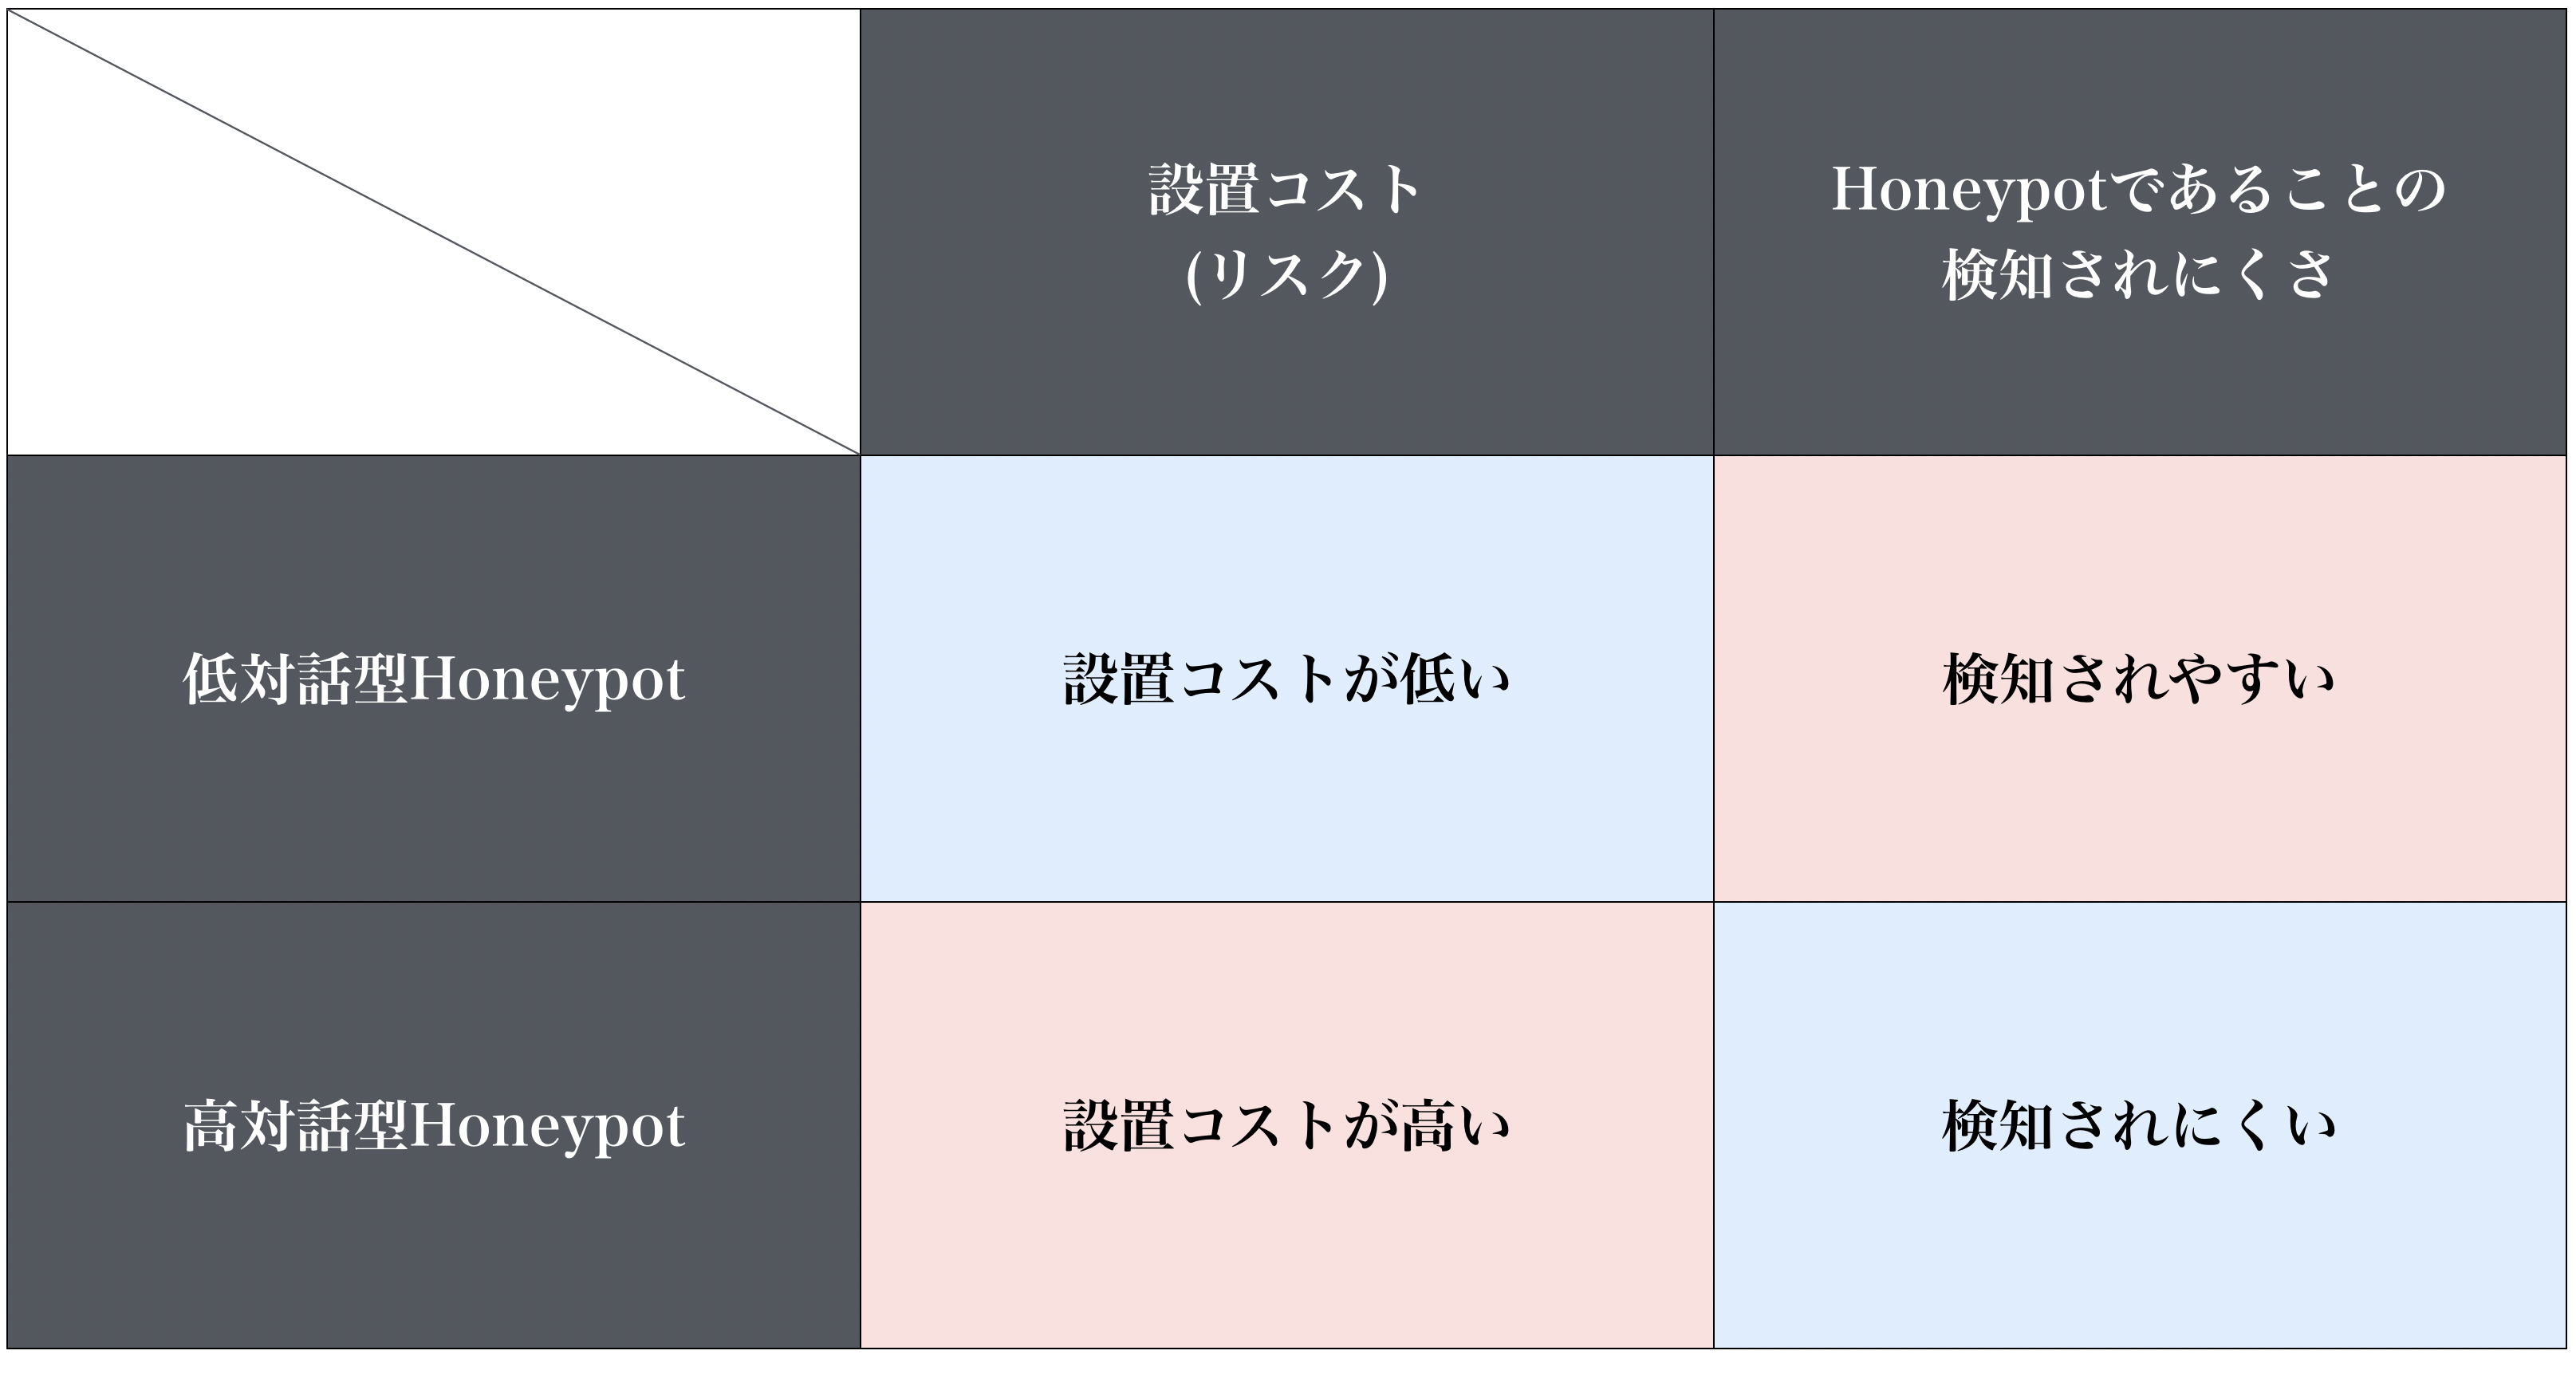
\includegraphics[width=1.0\textwidth]{figures/compare.png}
    \caption{SSHの低対話型HoneypotとSSHの高対話型Honeypotの比較}
    \label{fig:evo}
\end{figure}

%\begin{itemize}
%\setlength{\leftskip}{1.0cm}
% \item[危険責任] 製造者は製造物の設計図などの情報を消費者より詳細に知り得るため
% \item[報償責任] 製造者は製造物により利益を得るためそこから生じる責任を負うべきである
% \item[信頼責任] 製造者は自己の製品の安全性についてPRしており消費者はその品質が担保されているものであると期待する
%\end{itemize}

\section{Shell}
\label{tech:Shell}
ShellはOSのユーザーのためにインタフェースで,カーネルのサービスへのアクセスを提供するソフトウェアである.本研究での"Shell"はコマンドラインシェルのことを指す.

\subsection{Secure Shell}
\label{tech:Secure Shell}
Secure Shell(セキュアシェル、SSH)は、暗号や認証の技術を利用して、安全にリモートコンピュータと通信するためのプロトコルである.パスワードなどの認証部分を含むすべてのネットワーク上の通信が暗号化される.\cite{ssh}SSHにおける問題としては,通信する上での認証方法には鍵認証を推奨されているが,デフォルトではパスワード認証になっている.パスワード認証のままだとパスワードの総当たり攻撃を受けたり,パスワードが標準のままの設定であることで不正なログイン試行によって侵入を許してしまう.

\subsection{BusyBox}
\label{tech:BusyBox}
BusyBoxは標準UNIXコマンドで重要な多数のプログラムを単一のバイナリファイルに含むプログラムである.BusyBoxに含まれる,多数の標準UNIXコマンドで必要とするプログラムの実行ファイルは,LinuxというOSをBusyBoxだけでディストリビューションできるよう,"Linux上で最小の実行ファイル"として設計されている.一般にインストールされる実行ファイルは一部だけを実装できるように選択することができる.一般的にはBusyBoxのコマンドは200以上も用意されている.\cite{busybox}\footnote{今回使用したBusyBoxに含まれるコマンドの数は219}.
BusyBoxをインストールして実際に各コマンドを実行するためには,BusyBox内にある各コマンドにアクセス可能なようにpathを通すだけで良い.

\section{自然言語処理}
\label{tech:NLP}
人間が日常的に使っている自然言語をコンピュータに処理させる一連の技術である.本研究において,自然言語処理は意味解析のために使用した.意味解析には様々な手法があり,現在では大きくシソーラス解析とベクトル空間分析がある.

\subsection{シソーラス解析}
\label{tech:Siso}
シソーラスとは単語を意味レベルで分解し,抽象度の高いものから低いものへと遡っていくことができ,それを体系づけた類語辞書のことである.シソーラスには様々な言語において有名な辞書が存在する.有名なシソーラスとしてはPrinceton UniversityのWordNetがある.\cite{wordnet}

\subsubsection{Wordnet}
\label{tech:Wordnet}
WordNetは英単語がsynsetと呼ばれる同義語のグループに分類され,簡単な定義や,他の同義語のグループとの関係が記述されているデータベースである.WordNetのデータベースは約11万5000のsynsetに分類された約15万語を収録し,全体で20万3000の単語と意味の組み合わせがある.\cite{wordnetwiki}

\subsection{ベクトル空間解析}
\label{tech:Vector}
単語の意味を表現するため,単語の文章での出現回数や,その単語の周辺の単語をマトリクス上に表現することで,その単語を数学的に解釈できるようにしている.

\subsubsection{TF-IDF}
\label{tech:tfidf}
TFとはTerm Frequencyのことで,文章内での単語の出現頻度を表す.
数式で表すと以下のように表される.
\vspace{3mm}
\[
tf(t,d) = \frac{n_{t,d}}{\sum_{s \ni{d}}n_{s,d}}
\]
\vspace{3mm}
左辺の$ tf(t,d) $はTFの値で,文章d内に含まれる単語tの出現頻度を表す.
右辺の分子の$ n_{t,d} $は文章dにおける単語tの出現回数を表す.
右辺の分母の$ \sum_{s \ni{d}}n_{s,d} $は文章dにおける全ての単語の出現回数を表す.
つまり,
\vspace{3mm}
\[
\mbox{文章d内に含まれる単語tの出現頻度} = \frac{\mbox{文章dにおける単語tの出現回数}}{\mbox{文章dにおける全ての単語の出現回数}}
\]
\vspace{3mm}
を数式で表す.


\subsubsection{ベクトル空間モデル}
\label{tech:voctorkukan}

\subsubsection{Word2Vec}
\label{tech:Word2vec}



%%% Local Variables:
%%% mode: japanese-latex
%%% TeX-master: "../bthesis"
%%% End:
